% BEAMER ----
% This is just here so I know exactly what I'm looking at in Rstudio when messing with stuff.
\documentclass[10pt,ignorenonframetext,,aspectratio=149]{beamer}
\usetheme{metropolis}
\usefonttheme{serif} % use mainfont rather than sansfont for slide text
\setbeamertemplate{caption}[numbered]
\setbeamertemplate{caption label separator}{: }
\setbeamercolor{caption name}{fg=normal text.fg}
\usepackage{lmodern}
\usepackage{amssymb,amsmath}
\usepackage{ifxetex,ifluatex}
\usepackage{fixltx2e} % provides \textsubscript
\ifnum 0\ifxetex 1\fi\ifluatex 1\fi=0 % if pdftex
  \usepackage[T1]{fontenc}
  \usepackage[utf8]{inputenc}
\else % if luatex or xelatex
  \ifxetex
    \usepackage{mathspec}
  \else
    \usepackage{fontspec}
  \fi
  \defaultfontfeatures{Ligatures=TeX,Scale=MatchLowercase}
  \newcommand{\euro}{€}
    \setmainfont[]{Open Sans Light}
\fi
% use upquote if available, for straight quotes in verbatim environments
\IfFileExists{upquote.sty}{\usepackage{upquote}}{}
% use microtype if available
\IfFileExists{microtype.sty}{%
\usepackage{microtype}
\UseMicrotypeSet[protrusion]{basicmath} % disable protrusion for tt fonts
}{}
\usepackage{color}
\usepackage{fancyvrb}
\newcommand{\VerbBar}{|}
\newcommand{\VERB}{\Verb[commandchars=\\\{\}]}
\DefineVerbatimEnvironment{Highlighting}{Verbatim}{commandchars=\\\{\}}
% Add ',fontsize=\small' for more characters per line
\usepackage{framed}
\definecolor{shadecolor}{RGB}{248,248,248}
\newenvironment{Shaded}{\begin{snugshade}}{\end{snugshade}}
\newcommand{\AlertTok}[1]{\textcolor[rgb]{0.94,0.16,0.16}{#1}}
\newcommand{\AnnotationTok}[1]{\textcolor[rgb]{0.56,0.35,0.01}{\textbf{\textit{#1}}}}
\newcommand{\AttributeTok}[1]{\textcolor[rgb]{0.13,0.29,0.53}{#1}}
\newcommand{\BaseNTok}[1]{\textcolor[rgb]{0.00,0.00,0.81}{#1}}
\newcommand{\BuiltInTok}[1]{#1}
\newcommand{\CharTok}[1]{\textcolor[rgb]{0.31,0.60,0.02}{#1}}
\newcommand{\CommentTok}[1]{\textcolor[rgb]{0.56,0.35,0.01}{\textit{#1}}}
\newcommand{\CommentVarTok}[1]{\textcolor[rgb]{0.56,0.35,0.01}{\textbf{\textit{#1}}}}
\newcommand{\ConstantTok}[1]{\textcolor[rgb]{0.56,0.35,0.01}{#1}}
\newcommand{\ControlFlowTok}[1]{\textcolor[rgb]{0.13,0.29,0.53}{\textbf{#1}}}
\newcommand{\DataTypeTok}[1]{\textcolor[rgb]{0.13,0.29,0.53}{#1}}
\newcommand{\DecValTok}[1]{\textcolor[rgb]{0.00,0.00,0.81}{#1}}
\newcommand{\DocumentationTok}[1]{\textcolor[rgb]{0.56,0.35,0.01}{\textbf{\textit{#1}}}}
\newcommand{\ErrorTok}[1]{\textcolor[rgb]{0.64,0.00,0.00}{\textbf{#1}}}
\newcommand{\ExtensionTok}[1]{#1}
\newcommand{\FloatTok}[1]{\textcolor[rgb]{0.00,0.00,0.81}{#1}}
\newcommand{\FunctionTok}[1]{\textcolor[rgb]{0.13,0.29,0.53}{\textbf{#1}}}
\newcommand{\ImportTok}[1]{#1}
\newcommand{\InformationTok}[1]{\textcolor[rgb]{0.56,0.35,0.01}{\textbf{\textit{#1}}}}
\newcommand{\KeywordTok}[1]{\textcolor[rgb]{0.13,0.29,0.53}{\textbf{#1}}}
\newcommand{\NormalTok}[1]{#1}
\newcommand{\OperatorTok}[1]{\textcolor[rgb]{0.81,0.36,0.00}{\textbf{#1}}}
\newcommand{\OtherTok}[1]{\textcolor[rgb]{0.56,0.35,0.01}{#1}}
\newcommand{\PreprocessorTok}[1]{\textcolor[rgb]{0.56,0.35,0.01}{\textit{#1}}}
\newcommand{\RegionMarkerTok}[1]{#1}
\newcommand{\SpecialCharTok}[1]{\textcolor[rgb]{0.81,0.36,0.00}{\textbf{#1}}}
\newcommand{\SpecialStringTok}[1]{\textcolor[rgb]{0.31,0.60,0.02}{#1}}
\newcommand{\StringTok}[1]{\textcolor[rgb]{0.31,0.60,0.02}{#1}}
\newcommand{\VariableTok}[1]{\textcolor[rgb]{0.00,0.00,0.00}{#1}}
\newcommand{\VerbatimStringTok}[1]{\textcolor[rgb]{0.31,0.60,0.02}{#1}}
\newcommand{\WarningTok}[1]{\textcolor[rgb]{0.56,0.35,0.01}{\textbf{\textit{#1}}}}

% --------------------------------
% Separating this because this no
% longer works as of pandoc 3.2.1
% -------------------------------
%%\usepackage{graphicx,grffile}
%\makeatletter
%\def\maxwidth{\ifdim\Gin@nat@width>\linewidth\linewidth\else\Gin@nat@width\fi}
%\def\maxheight{\ifdim\Gin@nat@height>\textheight0.8\textheight\else\Gin@nat@height\fi}
%\makeatother
%% Scale images if necessary, so that they will not overflow the page
%% margins by default, and it is still possible to overwrite the defaults
%% using explicit options in \includegraphics[width, height, ...]{}
%\setkeys{Gin}{width=\maxwidth,height=\maxheight,keepaspectratio}
%
% ---------------------------------
% This works now: HT: Justin Esarey
% ---------------------------------
\usepackage{graphicx}
\makeatletter
\newsavebox\pandoc@box
\newcommand*\pandocbounded[1]{% scales image to fit in text height/width
  \sbox\pandoc@box{#1}%
  \Gscale@div\@tempa{\textheight}{\dimexpr\ht\pandoc@box+\dp\pandoc@box\relax}%
  \Gscale@div\@tempb{\linewidth}{\wd\pandoc@box}%
  \ifdim\@tempb\p@<\@tempa\p@\let\@tempa\@tempb\fi% select the smaller of both
  \ifdim\@tempa\p@<\p@\scalebox{\@tempa}{\usebox\pandoc@box}%
  \else\usebox{\pandoc@box}%
  \fi%
}
% Set default figure placement to htbp
\def\fps@figure{htbp}
\makeatother

% ^ saving this note in case I want some kind of conditional operation thingie.


% Comment these out if you don't want a slide with just the
% part/section/subsection/subsubsection title:
\AtBeginPart{
  \let\insertpartnumber\relax
  \let\partname\relax
  \frame{\partpage}
}
\AtBeginSection{
  \let\insertsectionnumber\relax
  \let\sectionname\relax
  \frame{\sectionpage}
}
\AtBeginSubsection{
  \let\insertsubsectionnumber\relax
  \let\subsectionname\relax
  \frame{\subsectionpage}
}

\setlength{\emergencystretch}{3em}  % prevent overfull lines
\providecommand{\tightlist}{%
  \setlength{\itemsep}{0pt}\setlength{\parskip}{0pt}}
\setcounter{secnumdepth}{0}

\title{Univariate Analysis}
\subtitle{IRIII.2 -- Quantitative Methods in the Study of International
Relations}
\author{Steven V. Miller}
\date{}


%% Here's everything I added.
%%--------------------------

\usepackage{graphicx}
\usepackage{rotating}
%\setbeamertemplate{caption}[numbered]
\usepackage{hyperref}
\usepackage{caption}
\usepackage[normalem]{ulem}
%\mode<presentation>
\usepackage{wasysym}
%\usepackage{amsmath}


% Get rid of navigation symbols.
%-------------------------------
\setbeamertemplate{navigation symbols}{}

% Optional institute tags and titlegraphic.
% Do feel free to change the titlegraphic if you don't want it as a Markdown field.
%----------------------------------------------------------------------------------
\institute{Department of Economic History and International Relations}

% \titlegraphic{\includegraphics[width=0.3\paperwidth]{\string~/Dropbox/teaching/clemson-academic.png}} % <-- if you want to know what this looks like without it as a Markdown field.
% -----------------------------------------------------------------------------------------------------
\titlegraphic{\vspace{6cm}\includegraphics[width=0.3\paperwidth]{/home/steve/Koofr/su/su-logotyp.png}}


% Some additional title page adjustments.
%----------------------------------------
\setbeamertemplate{title page}[empty]
%\date{}
\setbeamerfont{subtitle}{size=\small}

\setbeamercovered{transparent}

% Some optional colors. Change or add as you see fit.
%---------------------------------------------------
\definecolor{clemsonpurple}{HTML}{522D80}
 \definecolor{clemsonorange}{HTML}{F66733}
\definecolor{uiucblue}{HTML}{003C7D}
\definecolor{uiucorange}{HTML}{F47F24}

% new gig just dropped
\definecolor{sublue}{HTML}{002F5F}
\definecolor{susky}{HTML}{ACDEE6}
\definecolor{suwater}{HTML}{9BB2CE}





% Some optional color adjustments to Beamer. Change as you see fit.
%------------------------------------------------------------------
\setbeamercolor{frametitle}{fg=sublue,bg=white}
\setbeamercolor{title}{fg=sublue,,bg=white}
\setbeamercolor{local structure}{fg=sublue,}
\setbeamercolor{section in toc}{fg=sublue,bg=white}
% \setbeamercolor{subsection in toc}{fg=clemsonorange,bg=white}
\setbeamercolor{footline}{fg=sublue!50, bg=white}
\setbeamercolor{block title}{fg=sublue,bg=white}
\setbeamercolor{background canvas}{bg=white}


\setbeamercolor{title separator}{fg=suwater}

\let\Tiny=\tiny


% Sections and subsections should not get their own damn slide.
%--------------------------------------------------------------
\AtBeginPart{}
\AtBeginSection{}
\AtBeginSubsection{}
\AtBeginSubsubsection{}

% Suppress some of Markdown's weird default vertical spacing.
%------------------------------------------------------------
\setlength{\emergencystretch}{0em}  % prevent overfull lines
\setlength{\parskip}{0pt}


% Allow for those simple two-tone footlines I like.
% Edit the colors as you see fit.
%--------------------------------------------------
\defbeamertemplate*{footline}{my footline}{%
    \ifnum\insertpagenumber=1
    \hbox{%
        \begin{beamercolorbox}[wd=\paperwidth,ht=.8ex,dp=1ex,center]{}%
      % empty environment to raise height
        \end{beamercolorbox}%
    }%
    \vskip0pt%
    \else%
        \Tiny{%
            \hfill%
		\vspace*{1pt}%
            \insertframenumber/\inserttotalframenumber \hspace*{0.1cm}%
            \newline%
            \color{sublue}{\rule{\paperwidth}{0.4mm}}\newline%
            \color{suwater}{\rule{\paperwidth}{.4mm}}%
        }%
    \fi%
}

% Various cosmetic things, though I must confess I forget what exactly these do and why I included them.
%-------------------------------------------------------------------------------------------------------
\setbeamercolor{structure}{fg=blue}
\setbeamercolor{local structure}{parent=structure}
\setbeamercolor{item projected}{parent=item,use=item,fg=sublue,bg=white}
\setbeamercolor{enumerate item}{parent=item}

% Adjust some item elements. More cosmetic things.
%-------------------------------------------------
\setbeamertemplate{itemize item}{\color{sublue}$\bullet$}
\setbeamertemplate{itemize subitem}{\color{sublue}\scriptsize{$\bullet$}}
\setbeamertemplate{itemize/enumerate body end}{\vspace{.6\baselineskip}} % So I'm less inclined to use \medskip and \bigskip in Markdown.

% Automatically center images
% ---------------------------
% Note: this is for ![](image.png) images
% Use "fig.align = "center" for R chunks

\usepackage{etoolbox}

\AtBeginDocument{%
  \letcs\oig{@orig\string\includegraphics}%
  \renewcommand<>\includegraphics[2][]{%
    \only#3{%
      {\centering\oig[{#1}]{#2}\par}%
    }%
  }%
}

% I think I've moved to xelatex now. Here's some stuff for that.
% --------------------------------------------------------------
% I could customize/generalize this more but the truth is it works for my circumstances.

\ifxetex
\setbeamerfont{title}{family=\fontspec{Titillium Web}}
\setbeamerfont{frametitle}{family=\fontspec{Titillium Web}}
% Commented out -----
%\setbeamerfont{title}{family=\fontspec{Titillium Web}}
%\setbeamerfont{frametitle}{family=\fontspec{Titillium Web}}
\usepackage[font=small,skip=0pt]{caption}
 \else
 \fi

% {modelsummary} and {kableExtra} support
% --------------------------------------------------------------
% Rather than clutter my preambles for this stuff, it's just going to come by default.
\usepackage{dcolumn}
\usepackage{booktabs}
\usepackage{longtable}
\usepackage{array}
\usepackage{multirow}
\usepackage{wrapfig}
\usepackage{float}
\usepackage{colortbl}
\usepackage{pdflscape}
\usepackage{tabu}
\usepackage{threeparttable}


% Some random stuff now...
% ------------------------

\usepackage{tikz}

\newcommand{\shrug}[1][]{%
\begin{tikzpicture}[baseline,x=0.8\ht\strutbox,y=0.8\ht\strutbox,line width=0.125ex,#1]
\def\arm{(-2.5,0.95) to (-2,0.95) (-1.9,1) to (-1.5,0) (-1.35,0) to (-0.8,0)};
\draw \arm;
\draw[xscale=-1] \arm;
\def\headpart{(0.6,0) arc[start angle=-40, end angle=40,x radius=0.6,y radius=0.8]};
\draw \headpart;
\draw[xscale=-1] \headpart;
\def\eye{(-0.075,0.15) .. controls (0.02,0) .. (0.075,-0.15)};
\draw[shift={(-0.3,0.8)}] \eye;
\draw[shift={(0,0.85)}] \eye;
% draw mouth
\draw (-0.1,0.2) to [out=15,in=-100] (0.4,0.95);
\end{tikzpicture}}

% cols environment, for column-hackery.

\newenvironment{cols}[1][]{}{}

\newenvironment{col}[1]{\begin{minipage}{#1}\ignorespaces}{%
\end{minipage}
\ifhmode\unskip\fi
\aftergroup\useignorespacesandallpars}

\def\useignorespacesandallpars#1\ignorespaces\fi{%
#1\fi\ignorespacesandallpars}

\makeatletter
\def\ignorespacesandallpars{%
  \@ifnextchar\par
    {\expandafter\ignorespacesandallpars\@gobble}%
    {}%
}
\makeatother


% header includes go last.

\usepackage{dcolumn}
\usepackage{booktabs}
\usepackage{longtable}
\usepackage{array}
\usepackage{multirow}
\usepackage{wrapfig}
\usepackage{float}
\usepackage{colortbl}
\usepackage{pdflscape}
\usepackage{tabu}
\usepackage{threeparttable}

% Okay, and begin the actual document...

\begin{document}
\frame{\titlepage}

\section{Introduction}\label{introduction}

\begin{frame}{Goal(s) for Today}
\phantomsection\label{goals-for-today}
\begin{enumerate}
\tightlist
\item
  Introduce basic structure of the course
\item
  Emphasize the qualitative component of international relations.
\item
  Discuss some basic univariate methods/statistics you should know.
\end{enumerate}
\end{frame}

\begin{frame}{Course Information}
\phantomsection\label{course-information}
Hej! Jag heter Steve och jag talar inte mycket bra svenska. (Förlåt!)

\begin{itemize}
\tightlist
\item
  Mi español es aceptable como turista.
\item
  I'm also learning Korean.
\item
  (How about we do this in English instead\ldots)
\end{itemize}

Format: three lectures; seven labs

\begin{itemize}
\tightlist
\item
  See course description for more information about assignments
\item
  You can do these in Swedish (though I prefer English).
\end{itemize}

When in doubt, read the course description (it's 14 pages!)
\end{frame}

\section{Univariate Analysis}\label{univariate-analysis}

\subsection{Some Background to Get it Out of the
Way}\label{some-background-to-get-it-out-of-the-way}

\begin{frame}{Qualitative and Quantitative: What Are These Terms?}
\phantomsection\label{qualitative-and-quantitative-what-are-these-terms}
\textbf{Qualitative}: the analysis of \emph{non-numerical} data to
understand social phenomena

\bigskip

\textbf{Quantitative}: the analysis of \emph{numerical} data to
understand social phenomena
\end{frame}

\begin{frame}{Stages of Research}
\phantomsection\label{stages-of-research}
\begin{enumerate}
\setcounter{enumi}{-1}
\tightlist
\item
  Perspective
\item
  Causal theory
\item
  Hypothesis
\item
  Empirical test
\item
  Evaluation of hypothesis
\item
  Evaluation of causal theory
\item
  Advance in scientific knowledge
\end{enumerate}
\end{frame}

\begin{frame}{Perspective Matters}
\phantomsection\label{perspective-matters}
A perspective is a general orientation to the world. They're untestable
because:

\begin{enumerate}
\tightlist
\item
  They're too broad. Empirical support will never be total.
\item
  Perspectives are slippery and contextual.

  \begin{itemize}
  \tightlist
  \item
    e.g.~``People are rational.''
  \end{itemize}
\item
  Any empirical data observed can be interpreted to fit the perspective.
\end{enumerate}

We start with perspectives because we're not blank slates.
\end{frame}

\begin{frame}{Perspective Matters}
\phantomsection\label{perspective-matters-1}
A perspective is a general orientation to the world. They're untestable
because:

\begin{enumerate}
\tightlist
\item
  They're too broad. Empirical support will never be total.
\item
  Perspectives are slippery and contextual.

  \begin{itemize}
  \tightlist
  \item
    e.g.~``Government should stay out of our lives.''
  \end{itemize}
\item
  Any empirical data observed can be interpreted to fit the perspective.
\end{enumerate}

We start with perspectives because we're not blank slates.

\begin{itemize}
\tightlist
\item
  Rationality, for example, informs our general theories and the
  data-collection process.
\end{itemize}
\end{frame}

\subsection{Concepts and Measures}\label{concepts-and-measures}

\begin{frame}{Measuring a Conceptual World}
\phantomsection\label{measuring-a-conceptual-world}
Our world is fundamentally conceptual (qualitative)

\begin{itemize}
\tightlist
\item
  We start with an interest in concepts we observe (e.g.~``political
  tolerance'', ``corruption'', ``war'')
\item
  We devise a conceptual definition of what that thing is.
\item
  We \emph{operationalize} a definition of the thing to measure it.
\end{itemize}

From this, we get an empirical \emph{measure} of the concept.

\begin{itemize}
\tightlist
\item
  This allows us to proceed with political \emph{science}.
\end{itemize}
\end{frame}

\begin{frame}{Concept and Measure}
\phantomsection\label{concept-and-measure}
We seek to devise the best measure that best captures the ``true''
concept.

\begin{itemize}
\tightlist
\item
  However, there's always some slippage between concept and measure.
\item
  We do our best to eliminate as much error as we can.
\end{itemize}

There are two types of measurement error.

\begin{enumerate}
\tightlist
\item
  \textbf{Systematic measurement error}: the chronic, consistent
  distortion of a measure, leading to a \emph{mis}measure of the concept
  in question.
\item
  \textbf{Random measurement error}: haphazard, chaotic distortion of a
  measure, leading to an inconsistent operational reading of the
  concept.
\end{enumerate}
\end{frame}

\begin{frame}{Systematic Measurement Error Cases}
\phantomsection\label{systematic-measurement-error-cases}
Systematic measurement error is always the bigger concern of the two
because it can confound inference. Examples:

\begin{itemize}
\tightlist
\item
  Measuring ideology by party support.
\item
  Measuring corruption by mass-level perception of corruption (or by
  indicators like arrests).
\item
  Measuring human rights records with U.S. state department reports.
\end{itemize}

Detecting this is not always easy. You have to use your head.
\end{frame}

\begin{frame}{``Political Tolerance'' as a Classic Case}
\phantomsection\label{political-tolerance-as-a-classic-case}
\begin{figure}
\centering
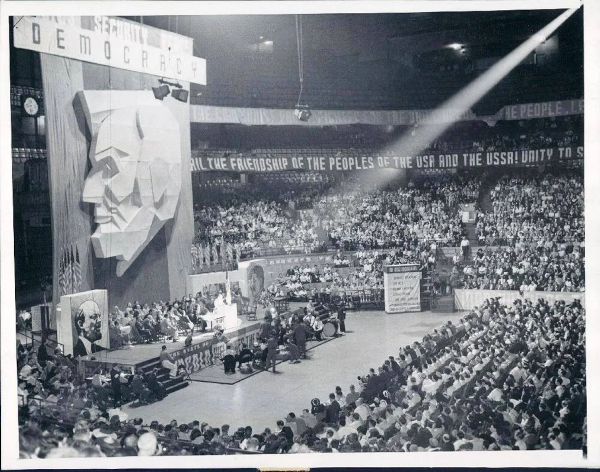
\includegraphics[width=0.7\linewidth,height=\textheight,keepaspectratio]{1938-05-27-communist-party-usa-convention.png}
\caption{Scenes from the Tenth Communist Party USA convention in Chicago
(May 1938)}
\end{figure}
\end{frame}

\begin{frame}{Validity and Reliability}
\phantomsection\label{validity-and-reliability}
This distinction maps nicely onto conversations about reliability and
validity.

\begin{itemize}
\tightlist
\item
  \textbf{Validity}: i.e.~am I measuring what I want without picking up
  anything else?
\item
  \textbf{Reliability}: am I consistently measuring what I want to
  measure?
\end{itemize}

Likewise, validity is the greater concern of the two.
\end{frame}

\subsection{Types of Variables}\label{types-of-variables}

\begin{frame}{Types of Variables}
\phantomsection\label{types-of-variables-1}
Assume you have a measure of your concept, you can summarize it any
number of ways.

\begin{itemize}
\tightlist
\item
  However, it's contingent on what information you're measure can
  communicate.
\end{itemize}
\end{frame}

\begin{frame}{The Classic Typology, for Better or Worse}
\phantomsection\label{the-classic-typology-for-better-or-worse}
The classic typology, a la Stanley Smith Stevens.

\begin{enumerate}
\tightlist
\item
  Nominal (i.e.~unordered-categorical)
\item
  Ordinal (i.e.~ordered-categorical)
\item
  Interval (i.e.~continuous)
\item
  Ratio (i.e.~continuous, but with meaningful zero as a kind of bound)
\end{enumerate}

There are important wrinkles to this, so let's get some examples.
\end{frame}

\begin{frame}{}
\phantomsection\label{section}
\begin{longtable}[t]{>{}c>{\raggedright\arraybackslash}p{30em}}
\caption{\label{tab:unnamed-chunk-1}GATT Members in Kono (2006)}\\
\toprule
\textbf{In GATT?} & \textbf{Countries}\\
\midrule
\textbf{0} & Albania, Algeria, Belarus, Bhutan, Estonia, Ethiopia, Kazakhstan, Kyrgyzstan, Latvia, Lithuania, Madagascar, Moldova, Nepal, Oman, PRC, Russia, Saudi Arabia\\
\textbf{1} & Argentina, Australia, Austria, Bangladesh, Bolivia, Brazil, Cameroon, Canada, Cent. Af. Rep., Chad, Chile, Costa Rica, Czech Rep., Ecuador, Egypt, El Salvador, Finland, Ghana, Guatemala, Honduras, Hungary, Iceland, India, Indonesia, Japan, Kenya, Malawi, Malaysia, Mauritius, Mexico, Morocco, Mozambique, New Zealand, Nicaragua, Nigeria, Norway, P. N. Guinea, Paraguay, Philippines, Poland, ROK, S. Africa, Singapore, Slovenia, Sri Lanka, Sweden, Switzerland, Tanzania, Thailand, Trinidad-Tobago, Tunisia, Turkey, USA, Uganda, Uruguay, Venezuela, Zambia, Zimbabwe\\
\bottomrule
\multicolumn{2}{l}{\rule{0pt}{1em}\textit{Note: }}\\
\multicolumn{2}{l}{\rule{0pt}{1em}FYI: You will see these data again in one of your problem sets.}\\
\end{longtable}
\end{frame}

\begin{frame}{}
\phantomsection\label{section-1}
\begin{longtable}[t]{lc}
\caption{\label{tab:unnamed-chunk-2}Groups in the EU Parliament from a 2024 Vote on Ukraine}\\
\toprule
\textbf{Group Label} & \textbf{No. of MEPs}\\
\midrule
European Conservatives and Reformists & 68\\
European People’s Party & 177\\
Greens/European Free Alliance & 72\\
Identity and Democracy & 59\\
Non-attached Members & 50\\
Progressive Alliance of Socialists and Democrats & 140\\
Renew Europe & 102\\
The Left in the European Parliament – GUE/NGL & 37\\
\bottomrule
\multicolumn{2}{l}{\rule{0pt}{1em}\textit{Note: }}\\
\multicolumn{2}{l}{\rule{0pt}{1em}Data: ?eu\_ua\_fta24 in \{stevedata\}}\\
\end{longtable}
\end{frame}

\begin{frame}{Unordered-Categorical Data}
\phantomsection\label{unordered-categorical-data}
Unordered-categorical data takes on a few forms.

\begin{itemize}
\tightlist
\item
  \emph{``Dummy'' variable}: has just two values.
\item
  \emph{Nominal variable}: has multiple values where one category is not
  the other.
\end{itemize}

Don't be fooled by order/information you perceive in a dummy variable.

\begin{itemize}
\tightlist
\item
  They're just a special case of a nominal variable.
\end{itemize}
\end{frame}

\begin{frame}{}
\phantomsection\label{section-2}
\begin{longtable}[t]{lccc}
\caption{\label{tab:unnamed-chunk-3}Financial Satisfaction in South Korea, 2023}\\
\toprule
\textbf{Financial Satisfaction} & \textbf{No.} & \textbf{Cum. Sum} & \textbf{\%}\\
\midrule
Very Dissatisfied & 59 & 59 & 5.25\%\\
Somewhat Dissatisfied & 271 & 330 & 29.39\%\\
Neither Satisfied nor Dissatisfied & 472 & 802 & 71.42\%\\
Somewhat Satisfied & 291 & 1093 & 97.33\%\\
Very Satisfied & 30 & 1123 & 100\%\\
\bottomrule
\multicolumn{4}{l}{\rule{0pt}{1em}\textit{Note: }}\\
\multicolumn{4}{l}{\rule{0pt}{1em}Data: Korean General Social Survey, 2023 (by way of ?kgss\_sample in \{simqi\}).}\\
\end{longtable}
\end{frame}

\begin{frame}{}
\phantomsection\label{section-3}
\pandocbounded{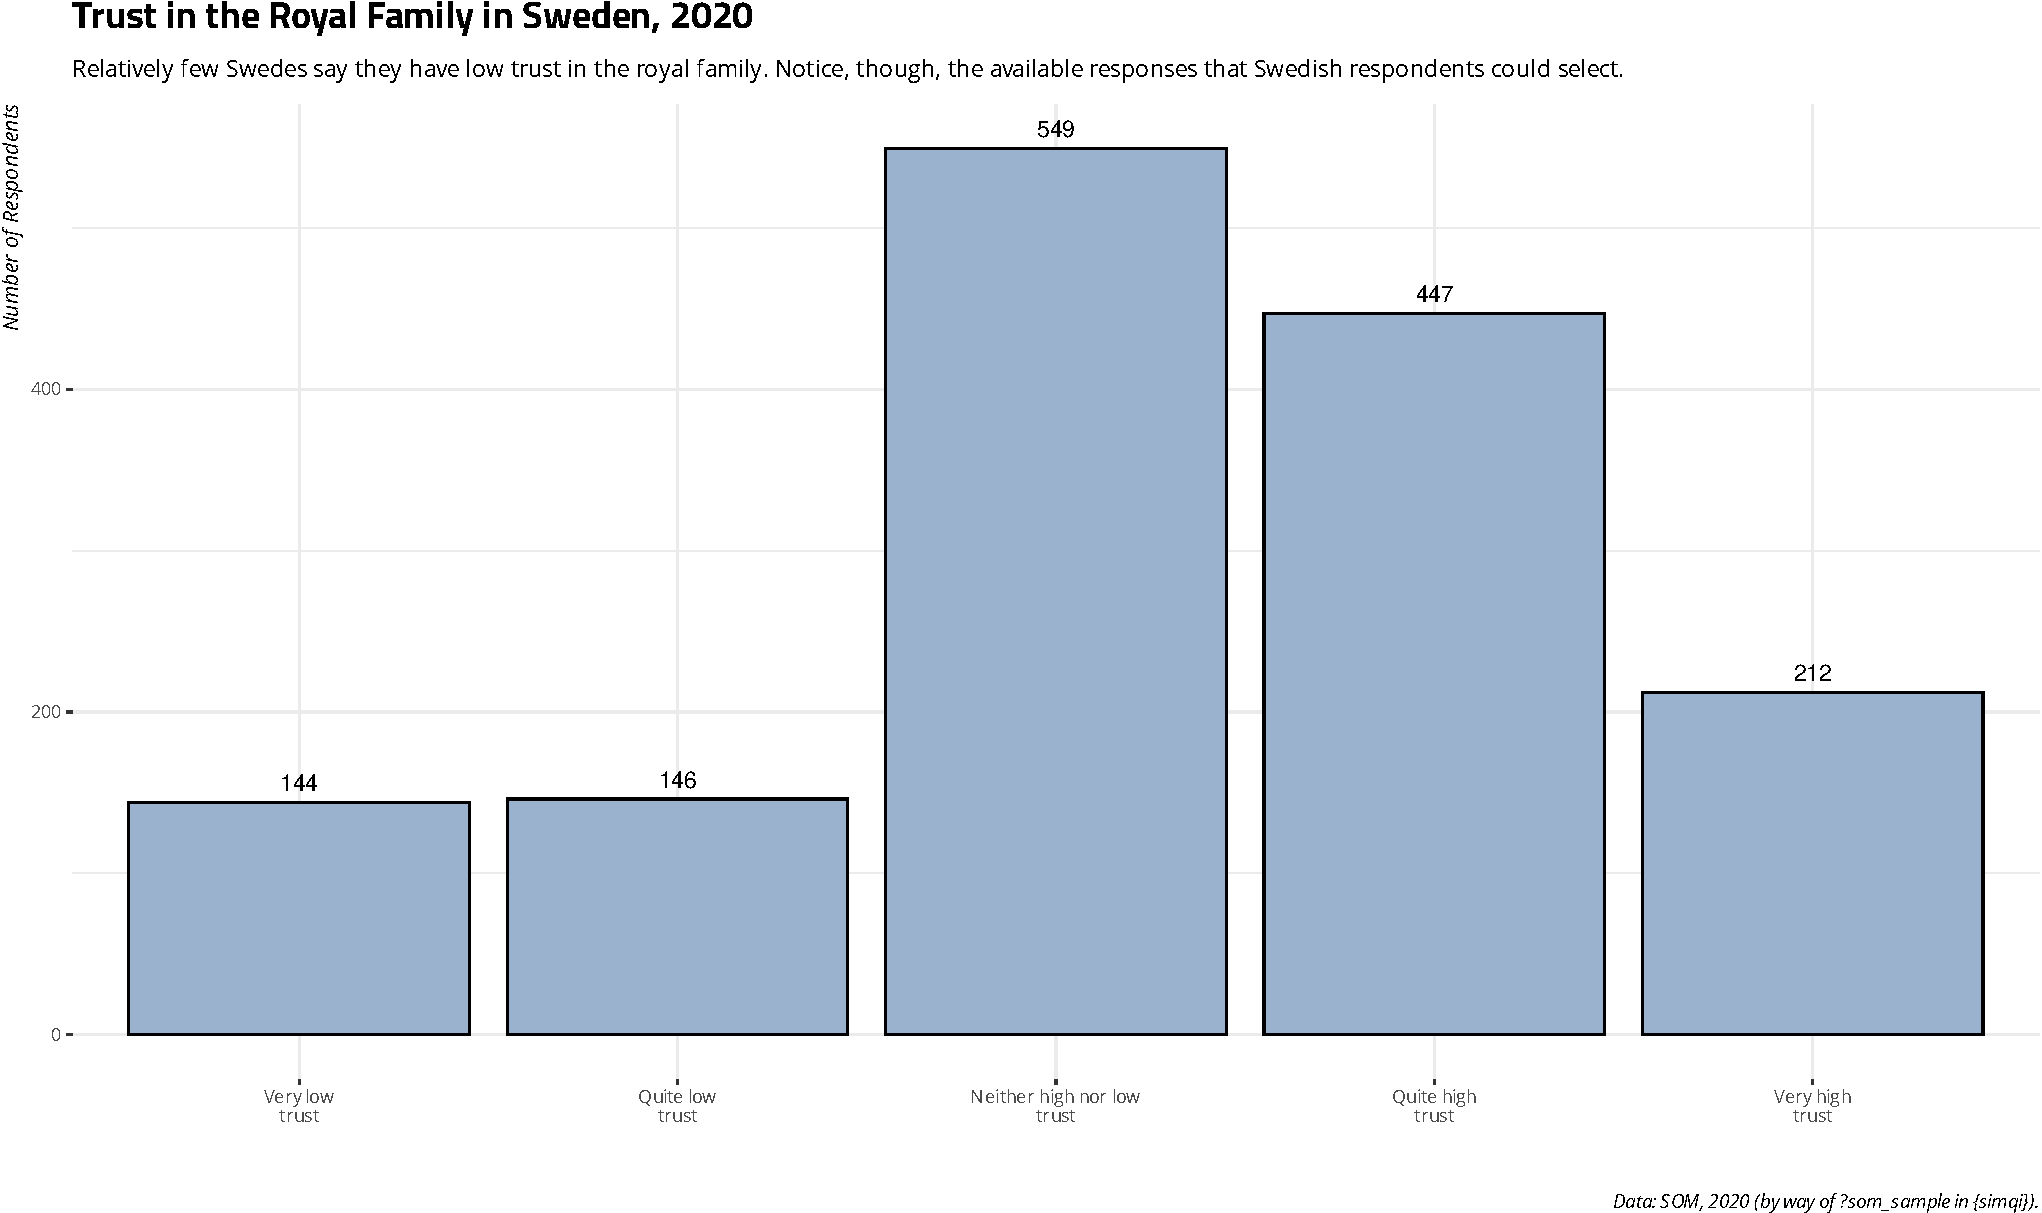
\includegraphics[keepaspectratio]{figs/unnamed-chunk-4.pdf}}
\end{frame}

\begin{frame}{Ordered-Categorical Data}
\phantomsection\label{ordered-categorical-data}
Ordered-categorical data have an order/rank, but:

\begin{itemize}
\tightlist
\item
  A finite set of available responses
\item
  No consistent difference between categories.
\end{itemize}

You'll see these kind of data often on:

\begin{itemize}
\tightlist
\item
  Questions of political support/trust/confidence
\item
  Likert items (with 5- or 7-point agree/disagree scale)
\item
  Assessments of political/financial satisfaction
\end{itemize}
\end{frame}

\begin{frame}{}
\phantomsection\label{section-4}
\pandocbounded{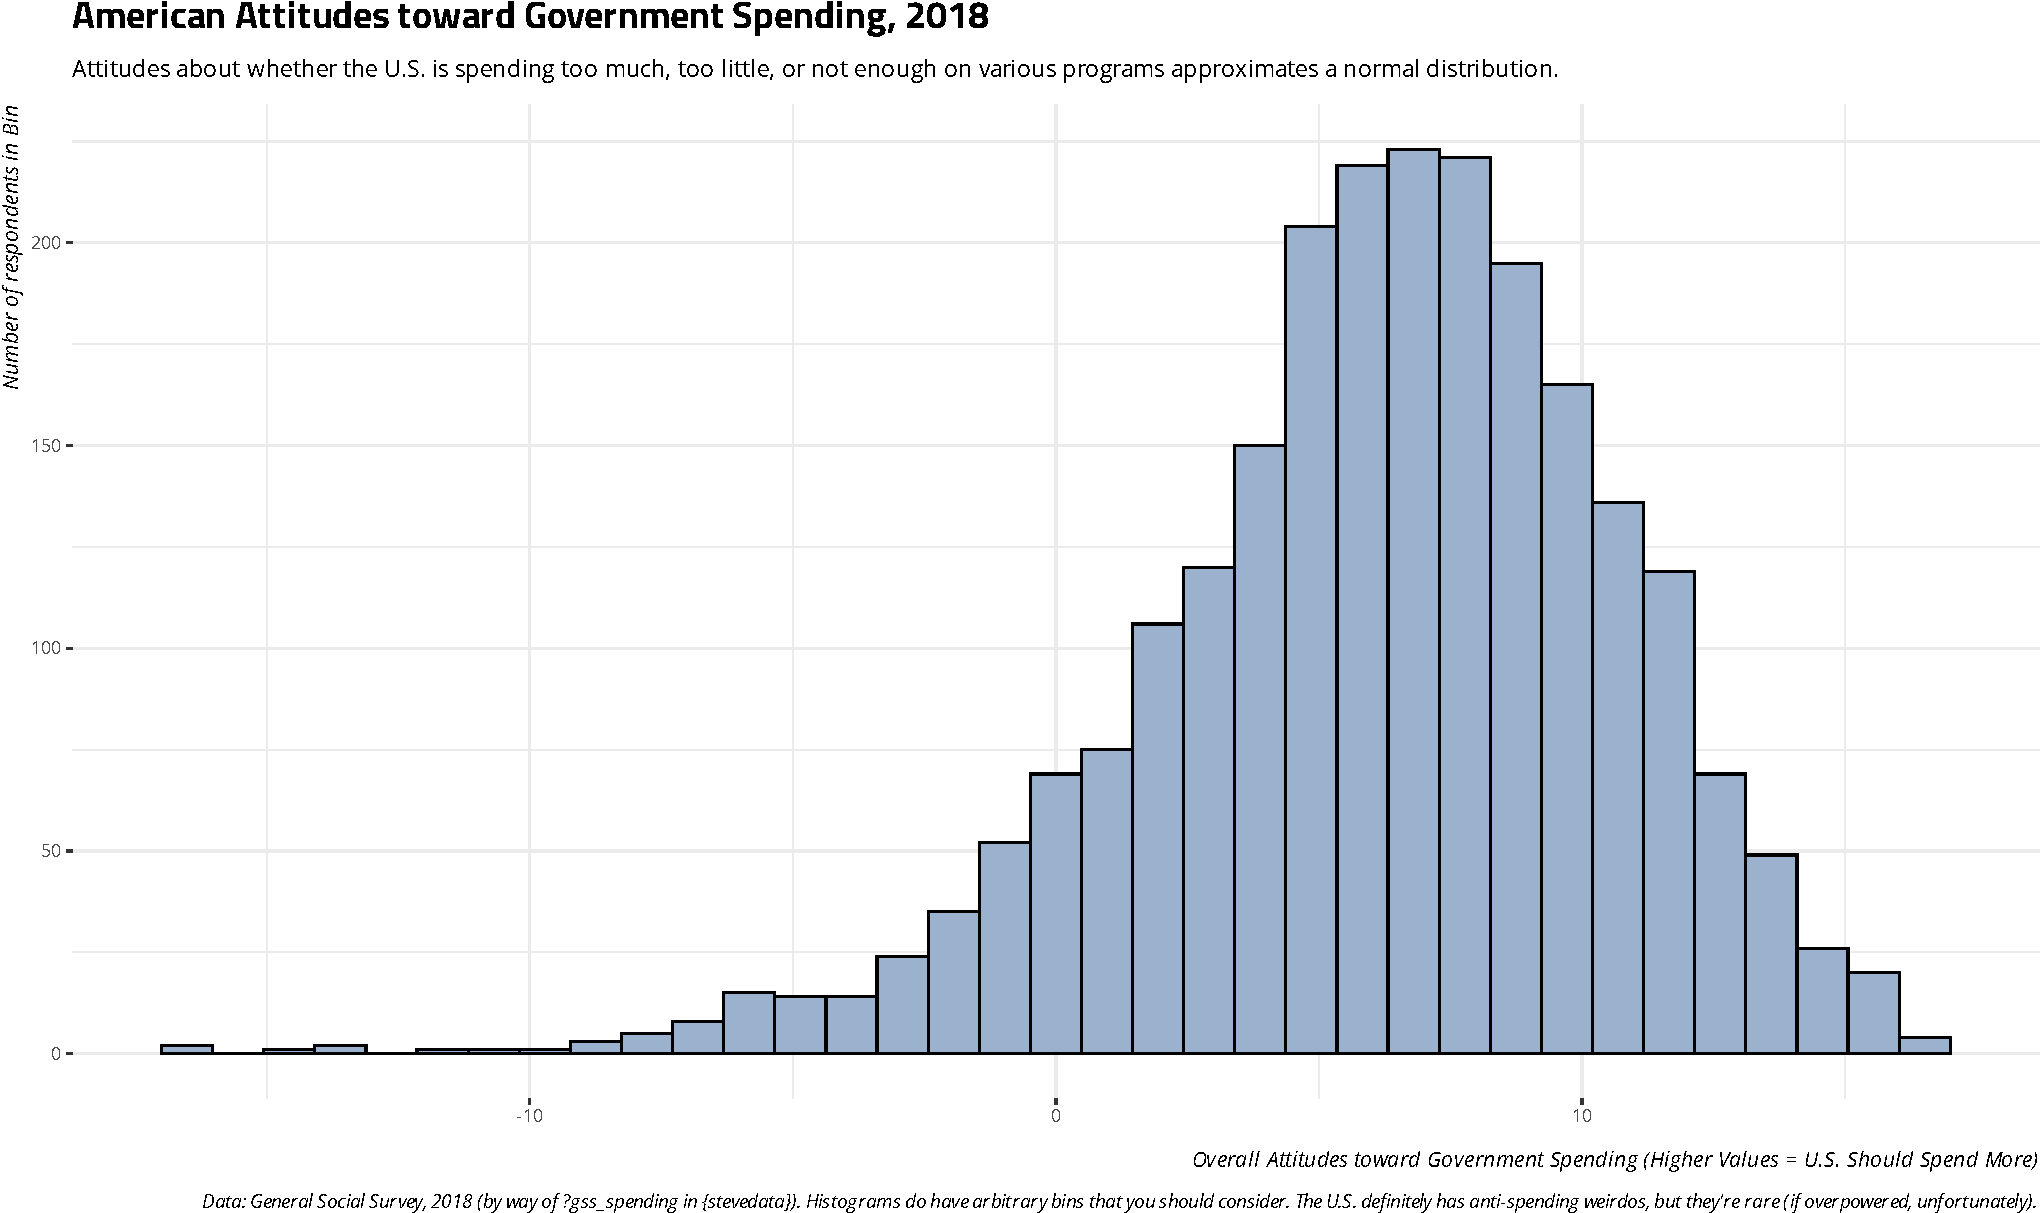
\includegraphics[keepaspectratio]{figs/unnamed-chunk-5.pdf}}
\end{frame}

\begin{frame}{}
\phantomsection\label{section-5}
\pandocbounded{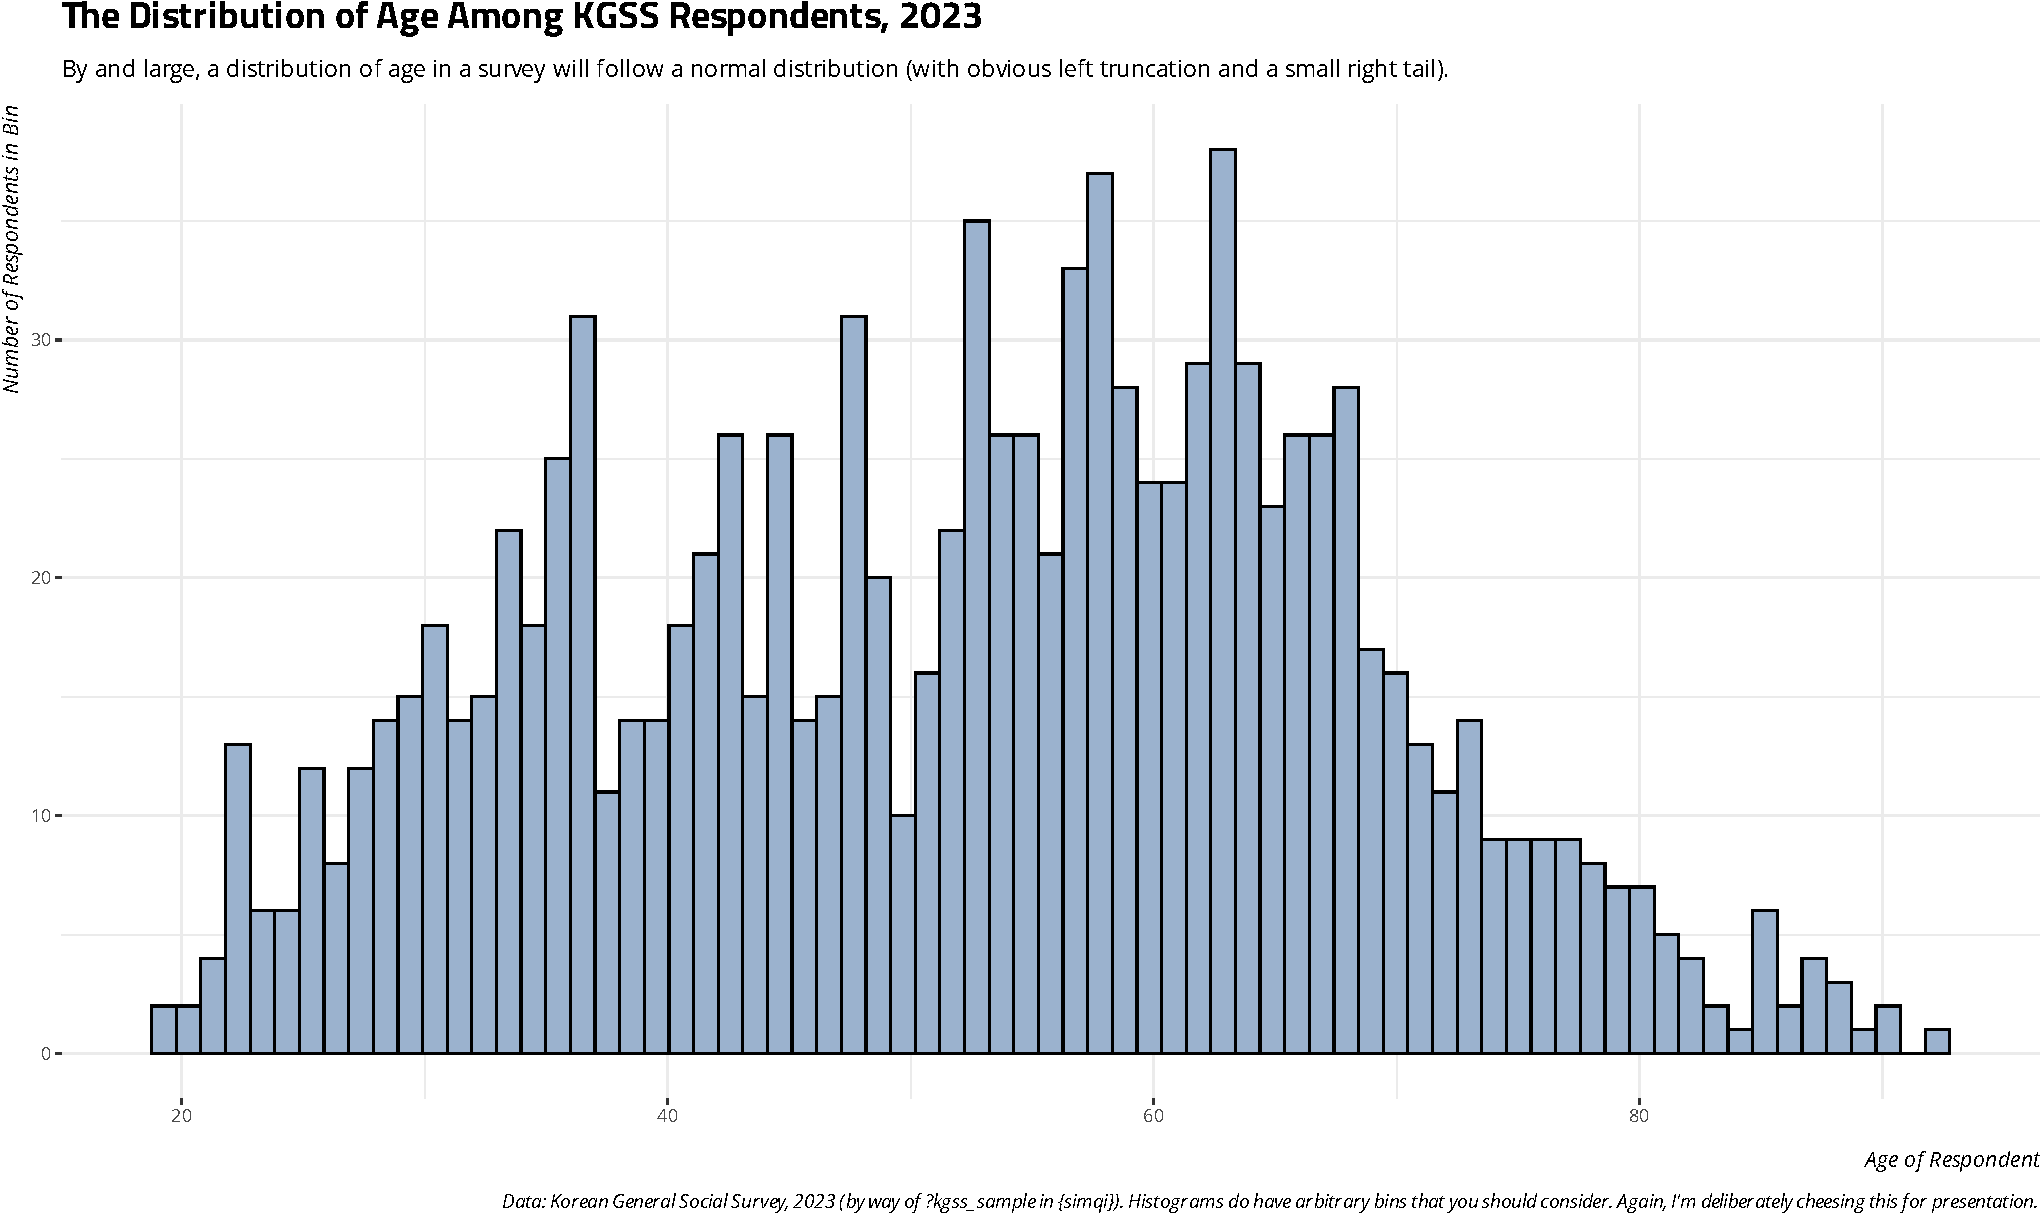
\includegraphics[keepaspectratio]{figs/unnamed-chunk-6.pdf}}
\end{frame}

\begin{frame}{}
\phantomsection\label{section-6}
\pandocbounded{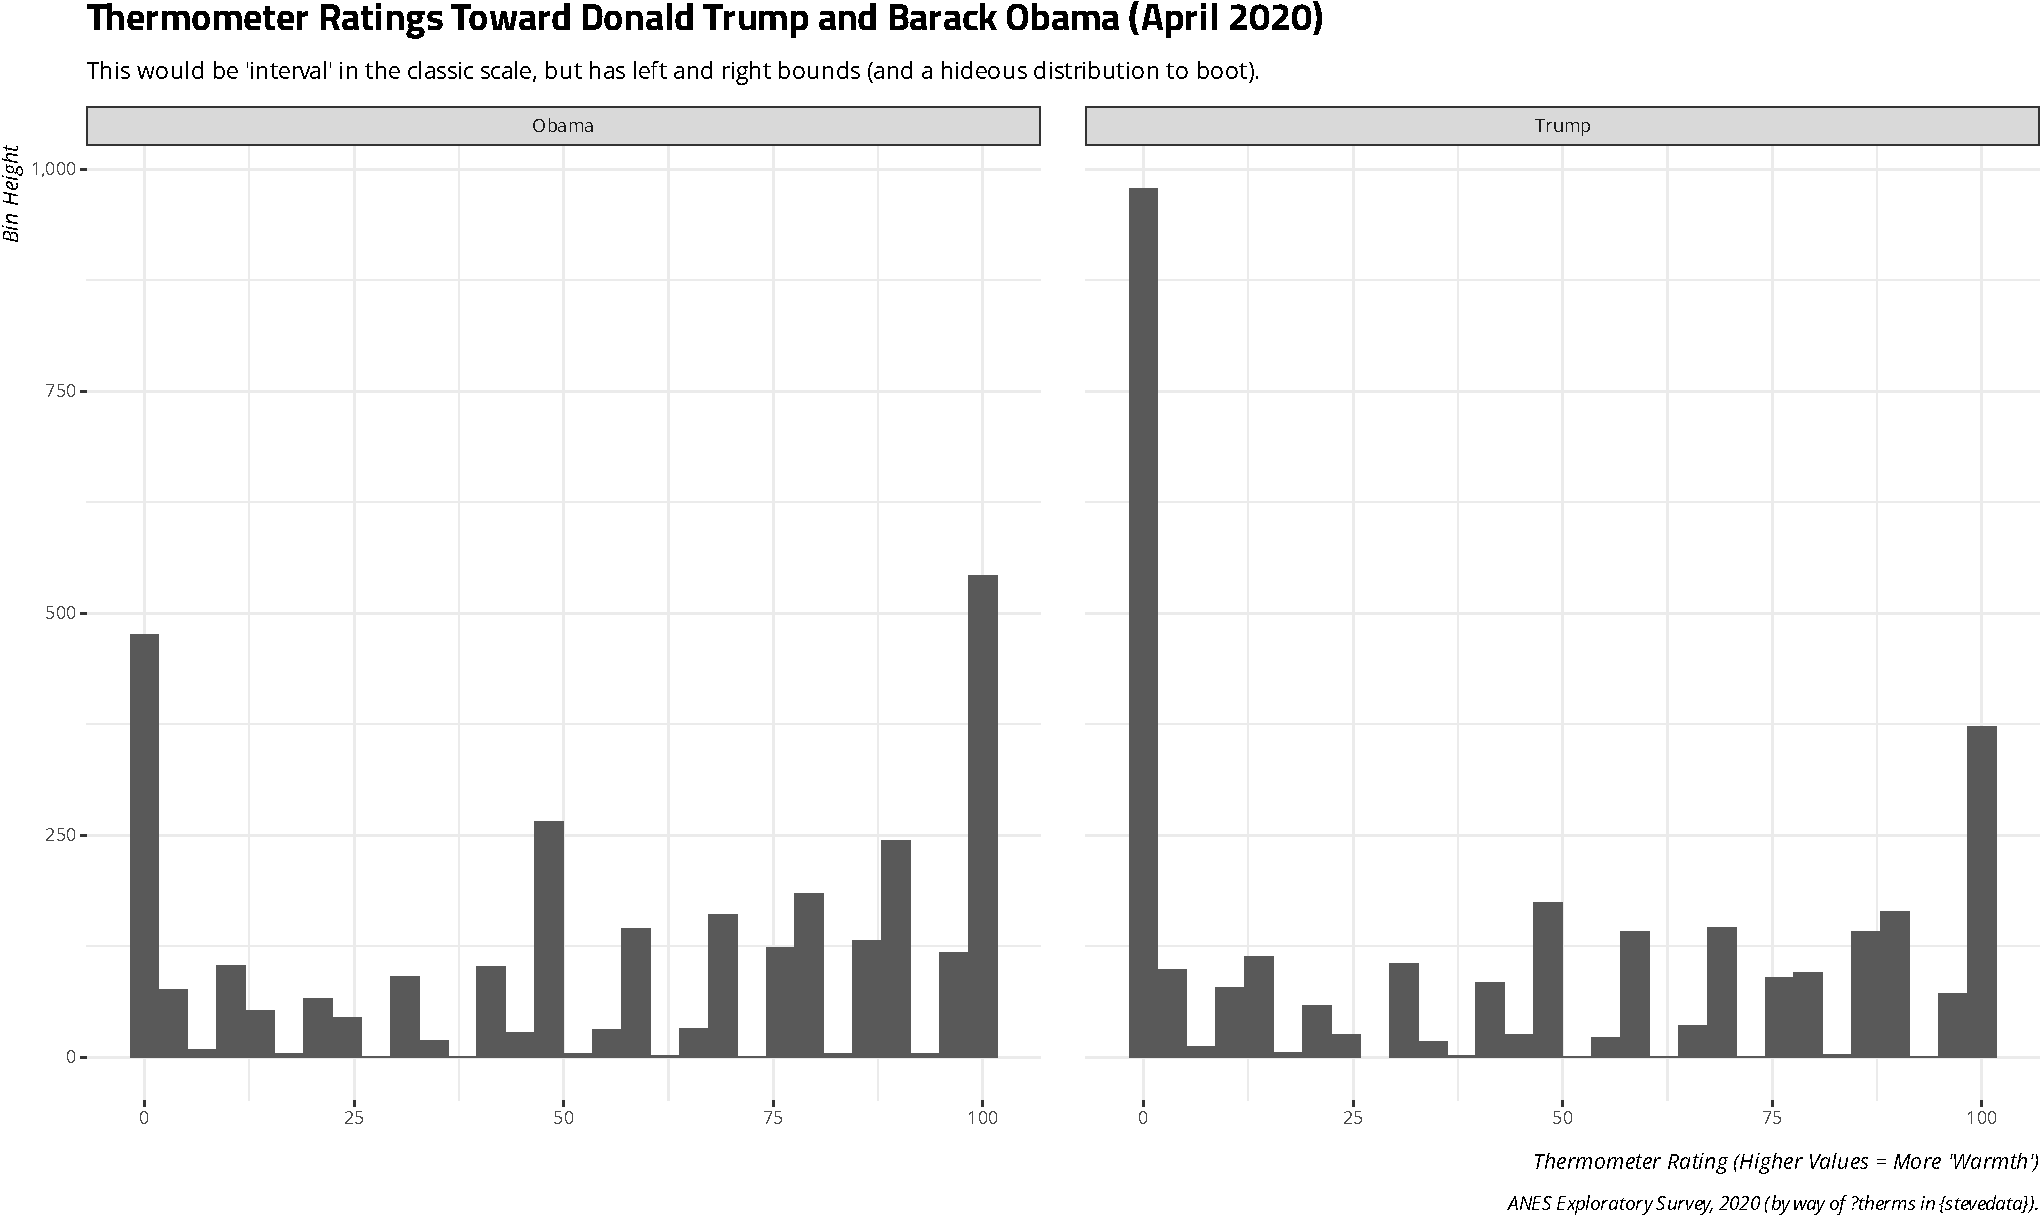
\includegraphics[keepaspectratio]{figs/unnamed-chunk-7.pdf}}
\end{frame}

\begin{frame}{}
\phantomsection\label{section-7}
\pandocbounded{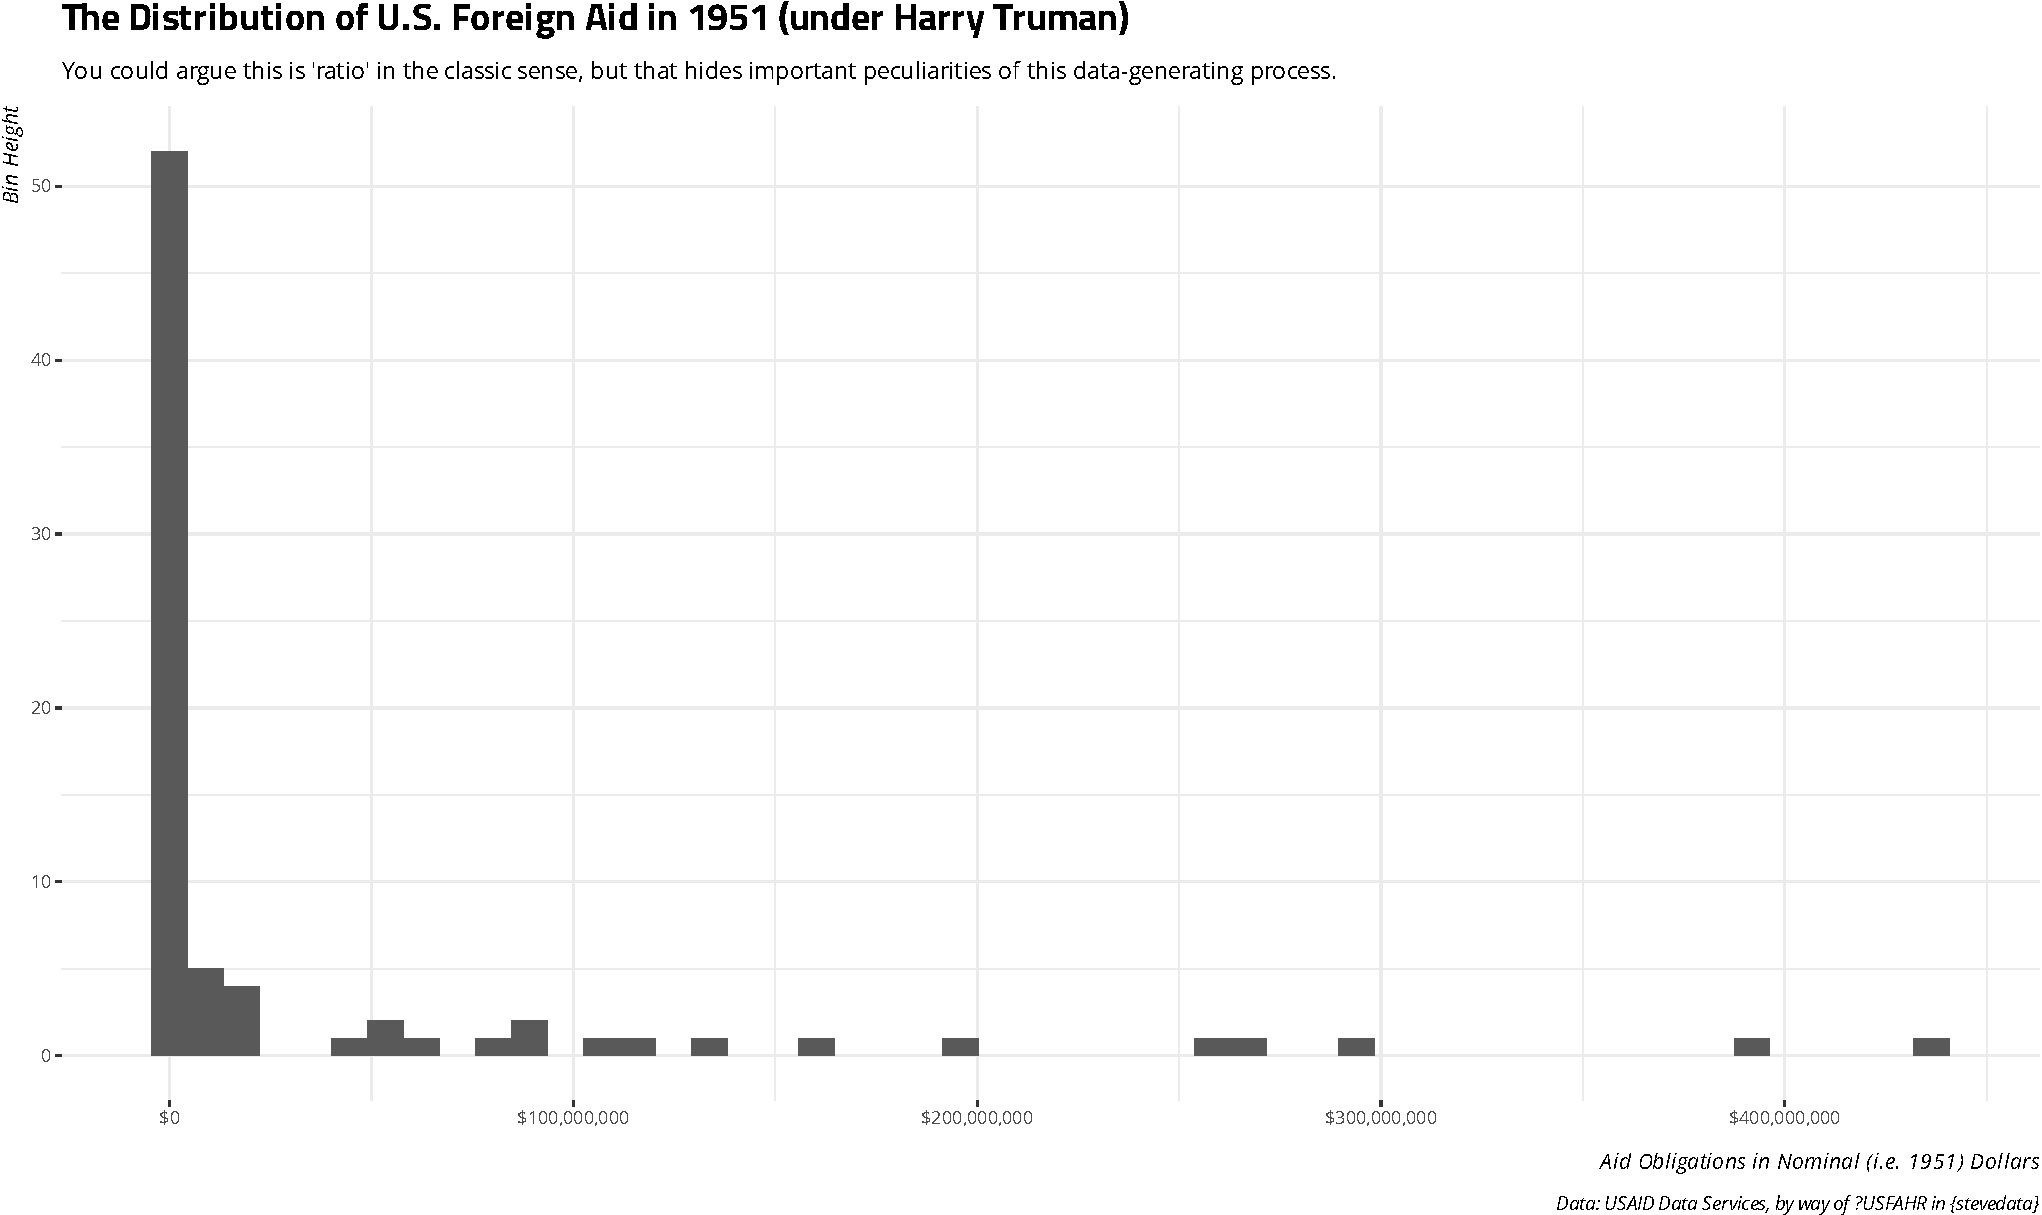
\includegraphics[keepaspectratio]{figs/unnamed-chunk-8.pdf}}
\end{frame}

\begin{frame}{Interval, Ratio, and Yadda Yadda Yadda}
\phantomsection\label{interval-ratio-and-yadda-yadda-yadda}
Both ``interval'' and ``ratio'' have granular (practically infinite)
possible values.

\begin{itemize}
\tightlist
\item
  In the classic typology, they are distinguished by what 0 means in the
  measure.
\end{itemize}

Rather than split these hairs, I'd encourage you to think of these as
``continuous''.

\begin{itemize}
\tightlist
\item
  i.e.~the values are infinitely (or practically) granular.
\item
  An arithmetic mean may not be faithful, but would make sense.

  \begin{itemize}
  \tightlist
  \item
    This even applies to some integers, like age and income.
  \end{itemize}
\end{itemize}
\end{frame}

\subsection{Summarizing Variables}\label{summarizing-variables}

\begin{frame}{Summarizing Variables}
\phantomsection\label{summarizing-variables-1}
\begin{longtable}[t]{lll}
\toprule
\textbf{Type} & \textbf{Central Tendency} & \textbf{Dispersion}\\
\midrule
Unordered-Categorical & Mode & (Some you'll use at an advanced level)\\
Ordered-Categorical & Median & IQR, MAD (Better to eyeball it)\\
'Continuous' & Mean & Standard Deviation\\
\bottomrule
\end{longtable}
\end{frame}

\begin{frame}{Identifying Measures of Central Tendency}
\phantomsection\label{identifying-measures-of-central-tendency}
\begin{longtable}[t]{lclc}
\caption{\label{tab:unnamed-chunk-10}County/Counties of Residence for Respondents in SOM (2019, 2020)}\\
\toprule
\textbf{County} & \textbf{No.} & \textbf{County} & \textbf{No.}\\
\midrule
Blekinge & 31 & Stockholm & 637\\
Dalarna & 92 & Södermanland & 73\\
Gävleborg & 75 & Uppsala & 88\\
Halland & 95 & Värmland & 77\\
Jämtland & 45 & Västerbotten & 88\\
Jönköping & 91 & Västernorrland & 61\\
Kalmar/Gotlands & 94 & Västmanland & 72\\
Kronoberg & 69 & Västra Götaland & 493\\
Norrbotten & 63 & Örebro & 83\\
Skåne & 383 & Östergötland & 131\\
\bottomrule
\multicolumn{4}{l}{\rule{0pt}{1em}\textit{Note: }}\\
\multicolumn{4}{l}{\rule{0pt}{1em}Data: SOM (2019 and 2020, by way of ?som\_sample in \{simqi\}).}\\
\end{longtable}
\end{frame}

\begin{frame}{Identifying Measures of Central Tendency}
\phantomsection\label{identifying-measures-of-central-tendency-1}
\begin{longtable}[t]{lccc}
\caption{\label{tab:unnamed-chunk-11}The Justifiability of Abortion in the U.S. in 2011}\\
\toprule
\textbf{Values} & \textbf{No.} & \textbf{Cum. Sum} & \textbf{Cum. Sum (\%)}\\
\midrule
Never Justifiable & 497 & 497 & 22.93\%\\
2 & 161 & 658 & 30.36\%\\
3 & 129 & 787 & 36.32\%\\
4 & 96 & 883 & 40.75\%\\
5 & 505 & 1388 & 64.05\%\\
6 & 154 & 1542 & 71.16\%\\
7 & 146 & 1688 & 77.9\%\\
8 & 176 & 1864 & 86.02\%\\
9 & 81 & 1945 & 89.76\%\\
Always Justifiable & 222 & 2167 & 100\%\\
\bottomrule
\multicolumn{4}{l}{\rule{0pt}{1em}\textit{Note: }}\\
\multicolumn{4}{l}{\rule{0pt}{1em}Data: World Values Survey, 2011 (by way of ?wvs\_usa\_abortion in \{stevedata\}.}\\
\end{longtable}
\end{frame}

\begin{frame}{Mean}
\phantomsection\label{mean}
The arithmetic \textbf{mean} is used only for continuous variables.

\begin{itemize}
\tightlist
\item
  This is to what we refer when we say ``average''.
\end{itemize}

Formally, \emph{i} through \emph{n}:

\begin{equation}
    \frac{1}{n}\Sigma x_i
\end{equation}

We can always describe continuous variables with the median.

\begin{itemize}
\tightlist
\item
  We cannot do the same for ordinal or nominal with the mean.
\item
  For really granular data, there is likely no real proper ``mode'' to
  report.
\end{itemize}
\end{frame}

\begin{frame}{}
\phantomsection\label{section-8}
\pandocbounded{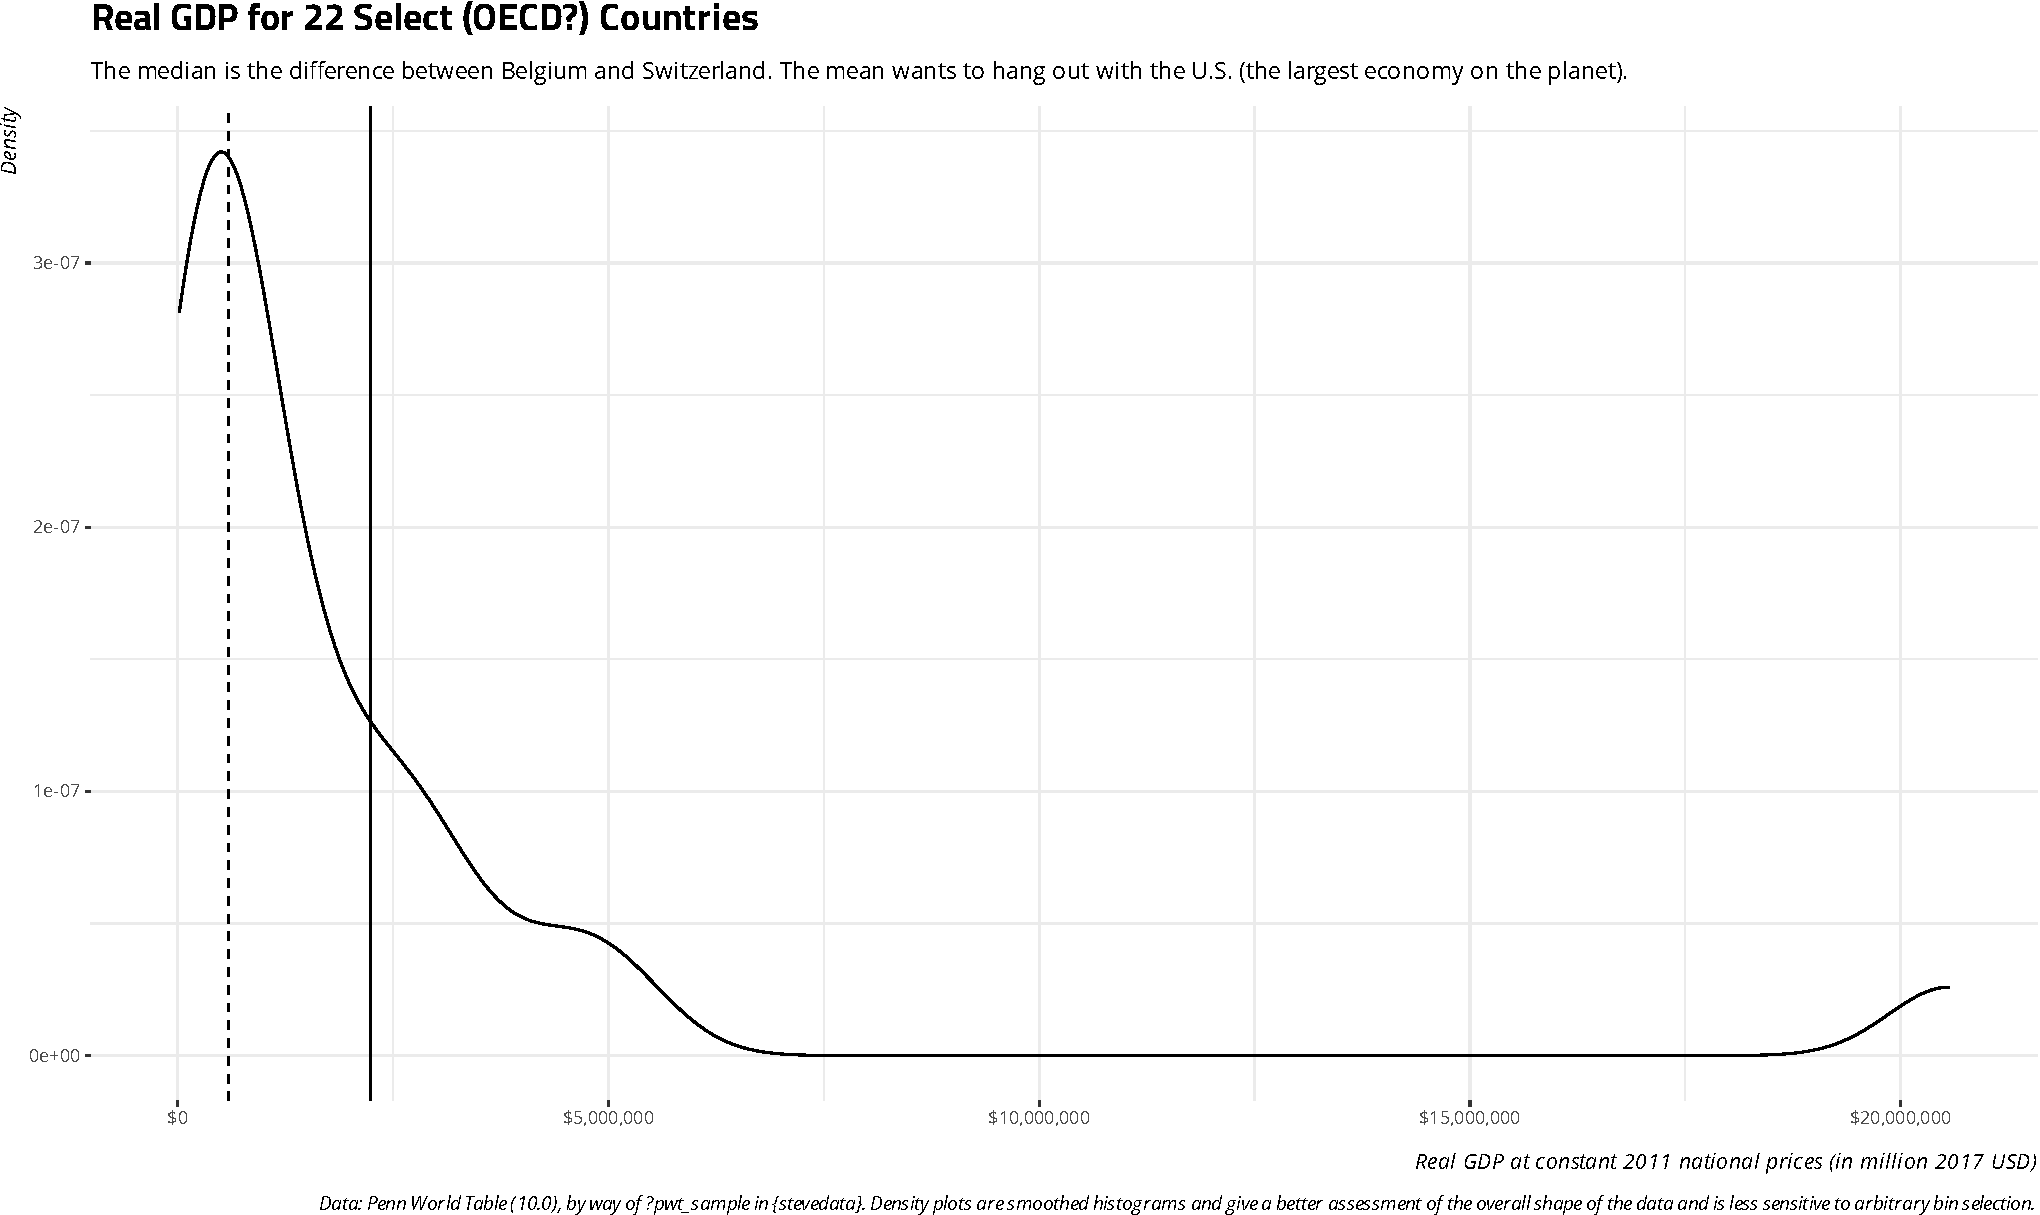
\includegraphics[keepaspectratio]{figs/unnamed-chunk-12.pdf}}
\end{frame}

\begin{frame}{A Comment on Dummy Variables}
\phantomsection\label{a-comment-on-dummy-variables}
Dummy variables behave curiously in measures of central tendency.

\begin{itemize}
\tightlist
\item
  Mode: most frequently occurring value (as it is nominal).
\item
  Median: also the mode.
\item
  Mean: the proportion of 1s.
\end{itemize}
\end{frame}

\begin{frame}{Dispersion}
\phantomsection\label{dispersion}
We also need to know variables by reference to its \textbf{dispersion}.

\begin{itemize}
\tightlist
\item
  i.e.~``how average is `average'?''
\item
  How far do variables deviate from the typical value?
\item
  If they do, measures of central tendency can be misleading.
\end{itemize}

In a lot of applications, you can just visualize this or look for a
table.

\begin{itemize}
\tightlist
\item
  If you have continuous data, you can get a precise measure: the
  \textbf{standard deviation}.

  \begin{itemize}
  \tightlist
  \item
    i.e.~the square root of the sum of squared deviations for each
    observation from the mean.
  \item
    There is a standard deviation for dummy variables, but it's
    different: \(\sqrt{p(1 - p)}\)
  \end{itemize}
\item
  For less precise data: just eye-ball it.

  \begin{itemize}
  \tightlist
  \item
    You could ask for an inter-quartile range or MAD, but, again,
    eye-ball it.
  \end{itemize}
\end{itemize}
\end{frame}

\begin{frame}[fragile]{How to Calculate a Standard Deviation}
\phantomsection\label{how-to-calculate-a-standard-deviation}
\begingroup\fontsize{7}{9}\selectfont

\begin{longtable}[t]{ccccccc>{}c}
\caption{\label{tab:unnamed-chunk-13}Calculating the Mean and Standard Deviation of Ten People's Age}\\
\toprule
\textbf{age} & \textbf{mean} & \textbf{dvtn} & \textbf{sum\_dvtn} & \textbf{dvtn2} & \textbf{sum\_dvtn2} & \textbf{variance} & \textbf{sd}\\
\midrule
41 & 36.3 & 4.7 & 0 & 22.09 & 266.1 & 29.567 & \textcolor{red}{\textbf{5.438}}\\
32 & 36.3 & -4.3 & 0 & 18.49 & 266.1 & 29.567 & \textcolor{red}{\textbf{\vphantom{1} 5.438}}\\
31 & 36.3 & -5.3 & 0 & 28.09 & 266.1 & 29.567 & \textcolor{red}{\textbf{5.438}}\\
32 & 36.3 & -4.3 & 0 & 18.49 & 266.1 & 29.567 & \textcolor{red}{\textbf{5.438}}\\
34 & 36.3 & -2.3 & 0 & 5.29 & 266.1 & 29.567 & \textcolor{red}{\textbf{5.438}}\\
40 & 36.3 & 3.7 & 0 & 13.69 & 266.1 & 29.567 & \textcolor{red}{\textbf{5.438}}\\
30 & 36.3 & -6.3 & 0 & 39.69 & 266.1 & 29.567 & \textcolor{red}{\textbf{5.438}}\\
35 & 36.3 & -1.3 & 0 & 1.69 & 266.1 & 29.567 & \textcolor{red}{\textbf{5.438}}\\
44 & 36.3 & 7.7 & 0 & 59.29 & 266.1 & 29.567 & \textcolor{red}{\textbf{\vphantom{1} 5.438}}\\
44 & 36.3 & 7.7 & 0 & 59.29 & 266.1 & 29.567 & \textcolor{red}{\textbf{5.438}}\\
\bottomrule
\end{longtable}
\endgroup{}

Alternatively:

\scriptsize

\begin{Shaded}
\begin{Highlighting}[]
\FunctionTok{sd}\NormalTok{(x)}
\CommentTok{\#\textgreater{} [1] 5.437524}
\end{Highlighting}
\end{Shaded}

\normalsize
\end{frame}

\section{Conclusion}\label{conclusion}

\begin{frame}{Please Install RStudio}
\phantomsection\label{please-install-rstudio}
\pandocbounded{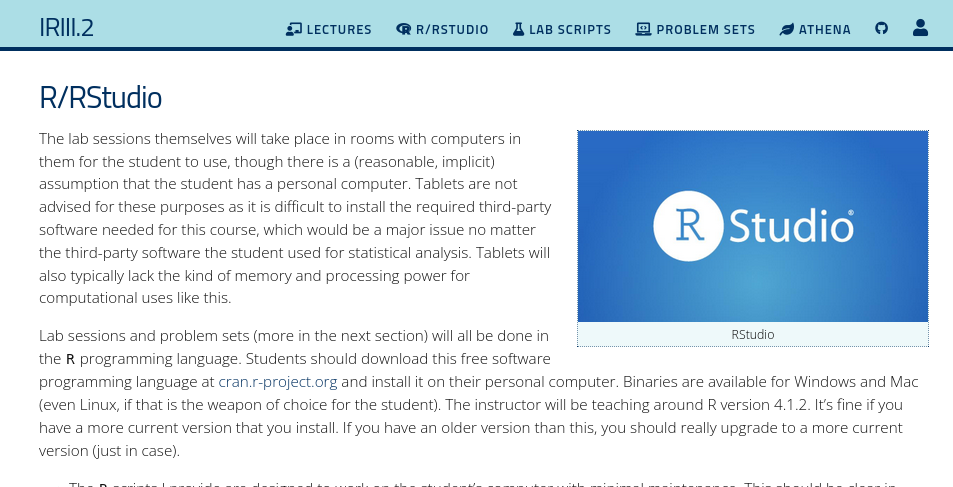
\includegraphics[keepaspectratio]{install-rstudio.png}}
\end{frame}

\begin{frame}{Conclusion}
\phantomsection\label{conclusion-1}
Welcome to IRIII.2 (the dungeon mini-boss of our program).

\begin{itemize}
\tightlist
\item
  All social science research is qualitative; some of it is
  quantitative.
\item
  Know your perspectives (i.e.~you have them, do trust).
\item
  There's always slippage (ideally random) between concept and measure.
\item
  Know your variable types and what information they communicate.
\end{itemize}
\end{frame}



\section[]{}
\frame{\small \frametitle{Table of Contents}
\tableofcontents}

\end{document}
